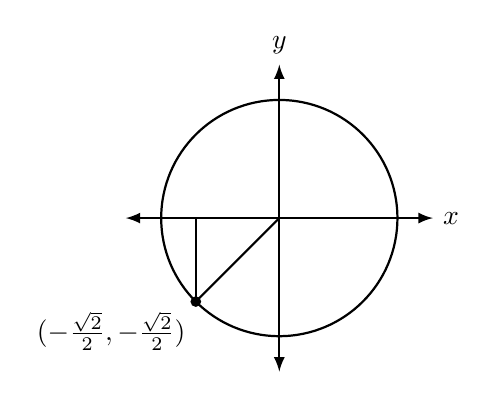
\begin{tikzpicture}[>=latex,scale=1.5,thick]
\draw [<->](-1.3,0)--(1.3,0) node [right] {$x$};
\draw [<->] (0,-1.3) -- (0,1.3) node [above] {$y$};
\draw (0,0) circle (1);
\draw [fill= black] (-.707,-.707) circle (1pt);
\draw (0,0) -- (-.707,-.707) node [below left] {$(-\frac{\sqrt{2}}{2}, -\frac{\sqrt{2}}{2})$};
\draw (-.707,-.707) -- (-.707,0);
\end{tikzpicture}

